\documentclass{article}

\usepackage{amssymb, amsmath, amsthm, graphicx, tikz, tikz-3dplot}
\usepackage{gensymb}
\usepackage[pdftitle = {Assignment 5},
  pdfauthor = {Cameron Fredrickson},
  pdfsubject = {Typesetting},
  colorlinks = true,
  urlcolor = blue,
  linkcolor = blue,
  citecolor = blue]{hyperref}

% tikz default degrees, r option in "cos(\x r)" specifies radians

\title{Assignment 5}
\author{Cameron Fredrickson}
\date{}

\begin{document}

\maketitle

\begin{enumerate}
    \item The graph of the function \(x^2 - x\) on \(\left[0, 3\right]\), with the are underneath the curve on \(\left[1, 2\right]\) representing the area calculated by \(\int_1^2 \left(x^2 - x \right) \, dx\).
    \begin{center}
    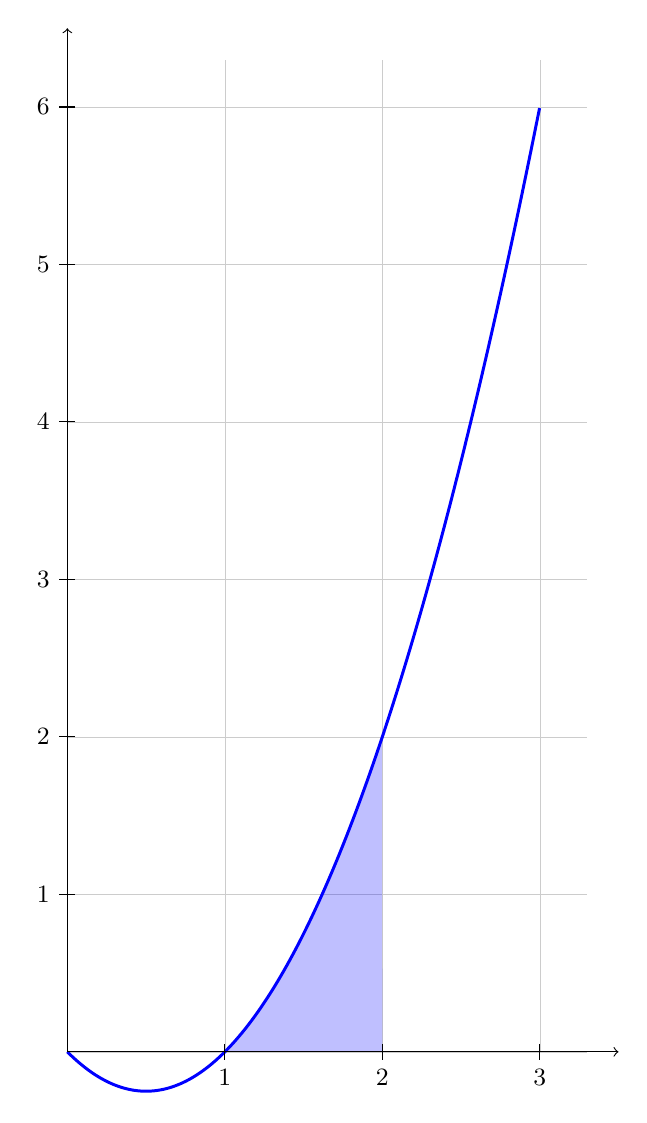
\begin{tikzpicture}[scale = 2]

    \draw [black!20, very thin] (0,0) grid (3.3,6.3);
    \fill [domain=1:2, smooth, blue, opacity = .25, samples = 100] (1,0) -- plot (\x, {pow(\x, 2) - \x}) -- (2,0) -- cycle;
    \draw [domain=0:3, smooth, line width = .25ex, blue, samples = 100] plot (\x, {pow(\x, 2) - \x});
    \draw [->, thin] (0,0) -- (0,6.5);
    \draw [->, thin] (0,0) -- (3.5,0);
    \foreach \x in {1,2,3,4,5,6} {
      \draw (.05, \x) -- (-.05, \x) node [left] {\begin{small}$\x$\end{small}};
    }
    \foreach \x in {1,2,3} {
      \draw (\x, .05) -- (\x, -.05) node [below] {\begin{small}$\x$\end{small}};
    }
    \end{tikzpicture}
    \end{center}

    \newpage

    \item Wikipedia states: \href{https://en.wikipedia.org/wiki/Wagner_graph}{In the mathematical field of graph theory, the Wagner Graph is a 3-regular graph with 8 verticies and 12 edges}. In a regular graph each vertex has the same number of neighbors, where vertex $B$ is a neighbor of vertex $A$ if vertex $B$ shares an edge with vertex $A$. Here is one representation of a Wagner Graph\footnote{To graph this I assumed the picture on \href{http://mathworld.wolfram.com/WagnerGraph.html}{Wolfram Alpha} was of a regular octogon (equiangular and equilateral) turned on it's side. I used simple trigonometry to find the interior angles of the polygon and the locations of the vertices}.
    \begin{center}
    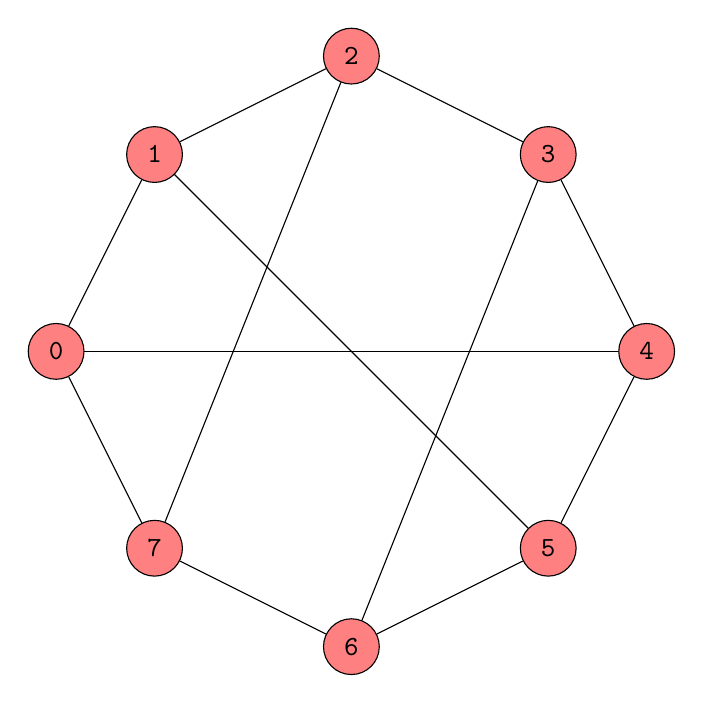
\begin{tikzpicture}[scale = 1.25]
    \tikzstyle{every node} = [draw, circle, fill = red!50, inner sep = 1ex];
    \node (v0) at (-3,0) {\texttt{0}};
    \node (v1) at (-2,2) {\texttt{1}};
    \node (v2) at (0,3.) {\texttt{2}};
    \node (v3) at (2,2) {\texttt{3}};
    \node (v4) at (3,0) {\texttt{4}};
    \node (v5) at (2,-2) {\texttt{5}};
    \node (v6) at (0,-3) {\texttt{6}};
    \node (v7) at (-2,-2) {\texttt{7}};
    \draw (v0) -- (v4);
    \draw (v1) -- (v5);
    \draw (v2) -- (v7);
    \draw (v3) -- (v6);
    \draw (v0) -- (v1);
    \draw (v1) -- (v2);
    \draw (v2) -- (v3);
    \draw (v3) -- (v4);
    \draw (v4) -- (v5);
    \draw (v5) -- (v6);
    \draw (v6) -- (v7);
    \draw (v7) -- (v0);
    \end{tikzpicture}
    \end{center}

\end{enumerate}

\end{document}